%!TEX encoding = UTF-8 Unicode
\documentclass[12pt]{article} 
\usepackage[left=0.75in,top=0.7in,right=0.75in,bottom=0.3in]{geometry} % Document margins
\usepackage{CJK}
\usepackage{graphicx}
\usepackage{mathtools}
\usepackage{mathrsfs}
\usepackage{amssymb}
\usepackage{hyperref}
\usepackage{sidecap}
\usepackage{makecell}
\usepackage{caption}

\makeatletter
\renewenvironment{itemize}
{\list{$\bullet$}{\leftmargin\z@ \labelwidth\z@ \itemindent-\leftmargin
\let\makelabel\descriptionlabel}}
{\endlist}
\makeatother

\begin{CJK}{UTF8}{bsmi}
\title{\textbf{VSP Final Project / Image Coding Contest}}
\author{\textbf{李豪韋 103061527} \\ \textbf{陳俐安 101061117}}
\date{}

\begin{document}
\vspace*{-60pt}
    {\let\newpage\relax\maketitle}

\vspace{-4em}
\section*{Overview}
\vspace{-20pt}
\noindent\makebox[\linewidth]{\rule{\textwidth}{0.4pt}}
\vspace{5pt}

The project is focused on images coding, especially lossy-coding, which is widely used in recent years. This document mainly consists of several sections: 1) implementation, which describes the ways we used in images coding in detail; 2) results, which demonstrates images after coding (real cases) and the evaluation plots (BD curve); 3) discussion, which contains something worth mentioning but is not required in the specification of project reports.

The source code is already publicly available on \href{https://github.com/HW-Lee/ImageCodec}{GitHub://HW-Lee/ImageCodec (hyperlink)}.

\section*{Implementation}
\vspace{-20pt}
\noindent\makebox[\linewidth]{\rule{\textwidth}{0.4pt}}

\begin{itemize}
	\item Coding Process
	\vspace{-1em}
	\begin{SCfigure}[][h]
		\vspace{-3em}
		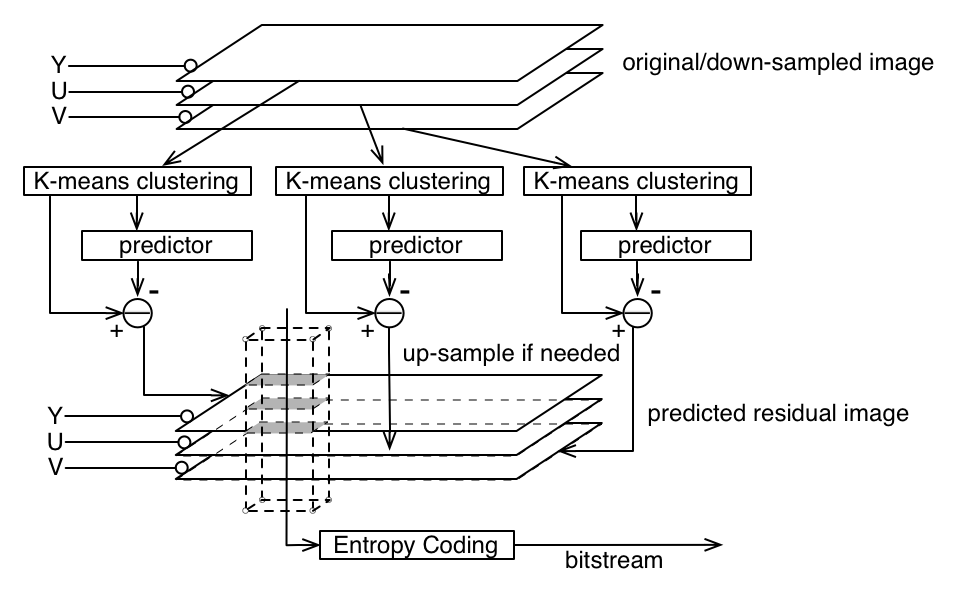
\includegraphics[scale=.35]{./res/codingProcessLevel1.png}
		\caption{level 1 coding, which uses 1) k-means clustering, to cluster YUV value for decreasing variance of values; 2) predictors, to intra-predict the image and coding residual to decreasing entropy; 3) up-sampler, to interpolate value in U/V such that Y/U/V contain the same width and height. It is main encoder of the system.}
	\end{SCfigure}
	\vspace*{-0em}
	\begin{SCfigure}[][h]
		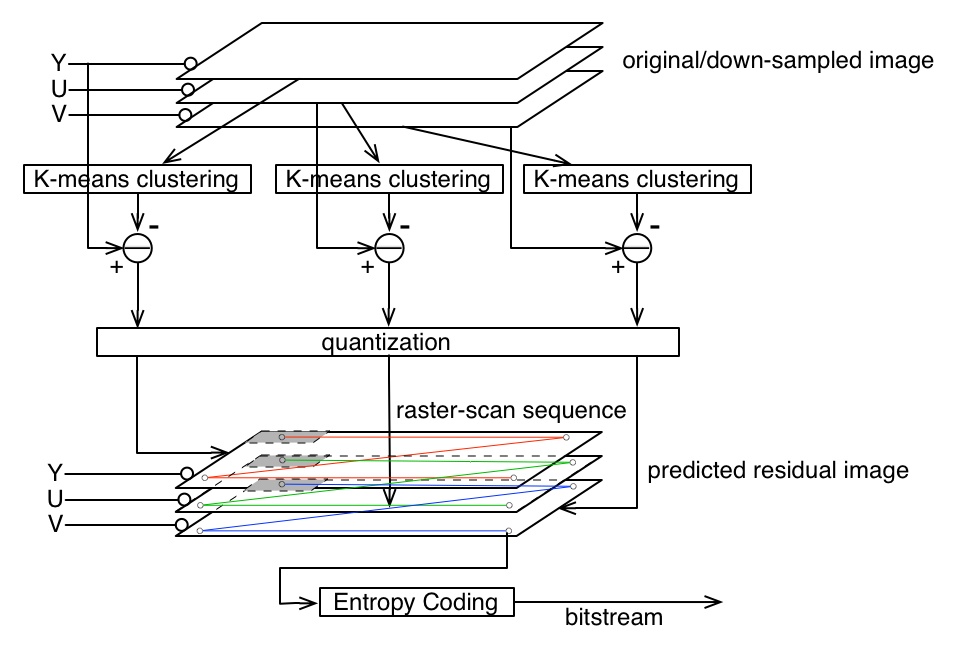
\includegraphics[scale=.35]{./res/codingProcessLevel2.png}
		\caption{level 2 coding (optional), which uses same components of level 1. It is optionally used for compensating PSNR caused by quantization, namely k-means clustering, and encodes the rest of information abandoned by level 1. Notice that this level still has a quantization process, brings more parametric flexibility to find a much better coding parameters.}
	\end{SCfigure}
	
	\newpage
	\item Coding Format Specification
		\begin{figure}[ht]
			\hspace*{-50pt}
			
\includegraphics[scale=.33]{./res/codingFormat.png}
			\caption{Coding format (top-to-bottom, left-to-right)}
		\end{figure}
	
	\item Methods Description
		\begin{enumerate}
			\item K-means clustering: reference from \href{https://en.wikipedia.org/wiki/K-means_clustering}{wiki: K-means\_clustering (hyperlink)}
				\begin{flushleft}
					The selected $K$ of Y/U/V (denoted $k_Y$/$k_U$/$k_V$) is power of 2, (e.g. $k_Y = 2^{m_Y}$, $m_Y \in \mathbb{Z}$) for purposes of 1) using the minimal number of bits to represent the maximal number of symbols; 2) controlling the number of bits per pixel. ($m = m_Y+m_U+m_V$)
				\end{flushleft}
			\item Negative values handling after subtraction
				\begin{flushleft}
					Even though the value range will be doubled after prediction (i.e. from $[0$, $2^N-1]$ to $[-2^N+1$, $2^N-1]$), it can still be mapped into $[0$, $2^N-1]$ fortunately. Therefore, 'circular subtraction' has been employed for making residual range keeps the same range as raw range. Circular subtraction is implemented with the mathematical form: $x \ominus_N y \equiv (x-y) \mod N$. \\
					Similarly, circular addition is also defined as $x \oplus_N y \equiv (x+y) \mod N$.
				\end{flushleft}
			\item Entropy coding: encoded with \href{https://en.wikipedia.org/wiki/Canonical_Huffman_code}{Canonical Huffman Coding (hyperlink)}
				\begin{flushleft}
					The codebook in level 1 consists of symbols which represent information of a pixel, but that in level 2 consists of symbols which represent information of a component. (raster-scan order)
				\end{flushleft}
			\item Down-sampling: for low-bitrate constraints, down-sample the image before encoding.
				\begin{flushleft}
					The way choosing the representative value: find the median in each $\text{dsr}_w \times \text{dsr}_h$ block.
				\end{flushleft}
			\item Predictors: use adjacent previous blocks (A, B, C) to predict the current block (D).
				\begin{figure}[ht]
					\centering
					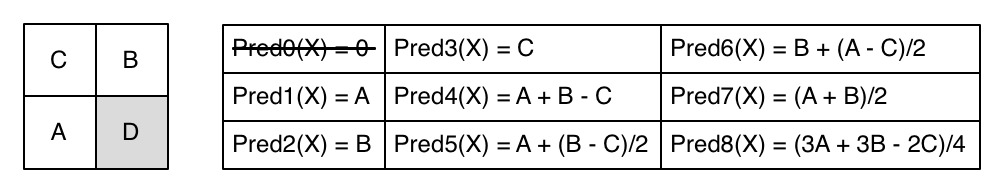
\includegraphics[scale=.4]{./res/predictors.png}
					\vspace*{-2.5em}
				\end{figure}
		\end{enumerate}
\end{itemize}

\section*{Results}
\vspace{-20pt}
\noindent\makebox[\linewidth]{\rule{\textwidth}{0.4pt}}

\begin{enumerate}
	\item Sample Image (see more on \href{https://github.com/HW-Lee/ImageCodec/tree/master/results}{GitHub://HW-Lee/ImageCodec/results (hyperlink)})
		\begin{figure}[ht]
			\begin{minipage}[c]{0.48\linewidth}
				\centering
				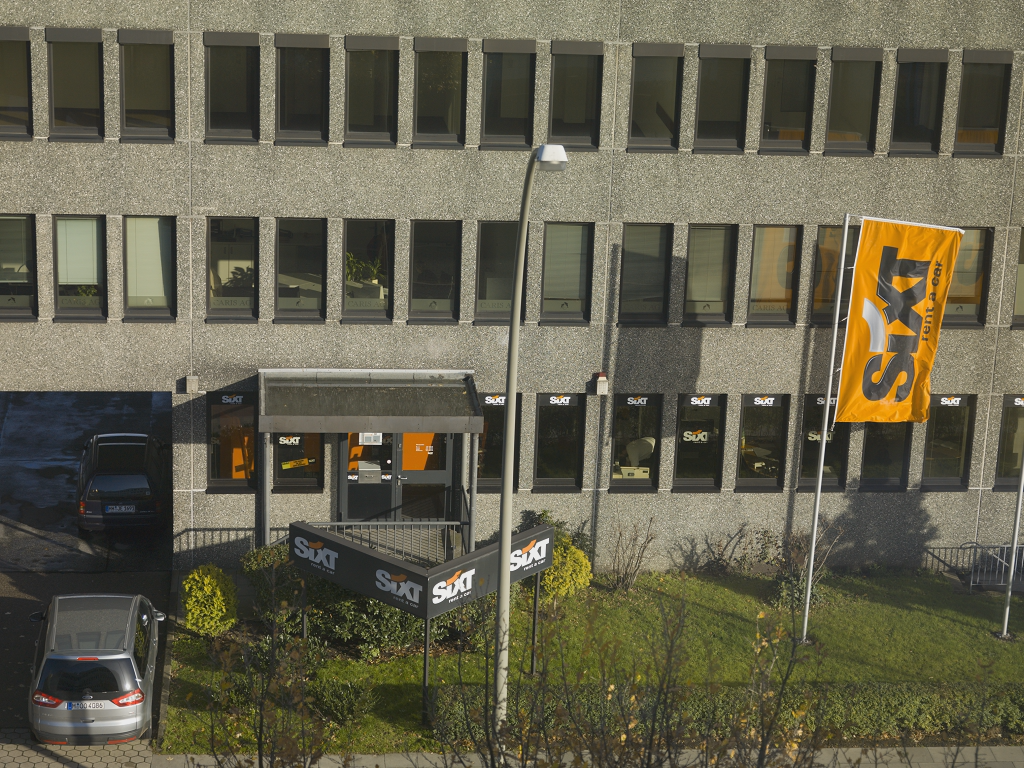
\includegraphics[scale=.23]{./res/sample_image/original.png}
				\caption*{original image}
				\vspace{10pt}
				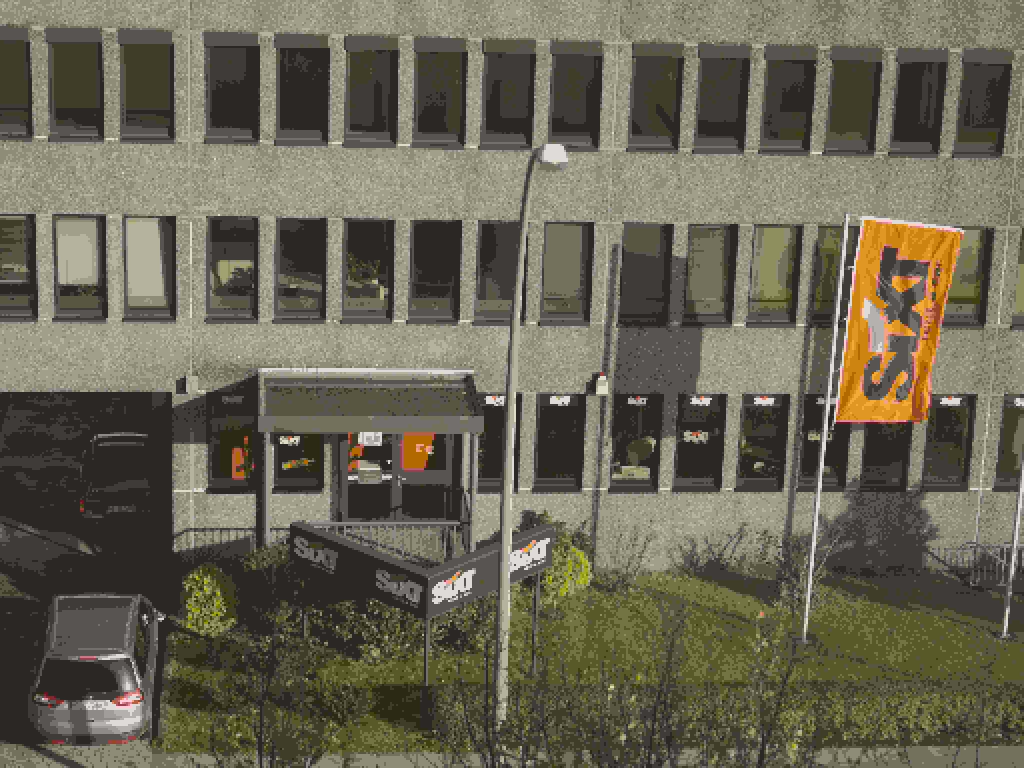
\includegraphics[scale=.23]{./res/sample_image/decompressed1.png}
				\caption*{bitrate: 0.5075, PSNR: 26.9286}
			\end{minipage}
			\begin{minipage}[c]{0.48\linewidth}
				\centering
				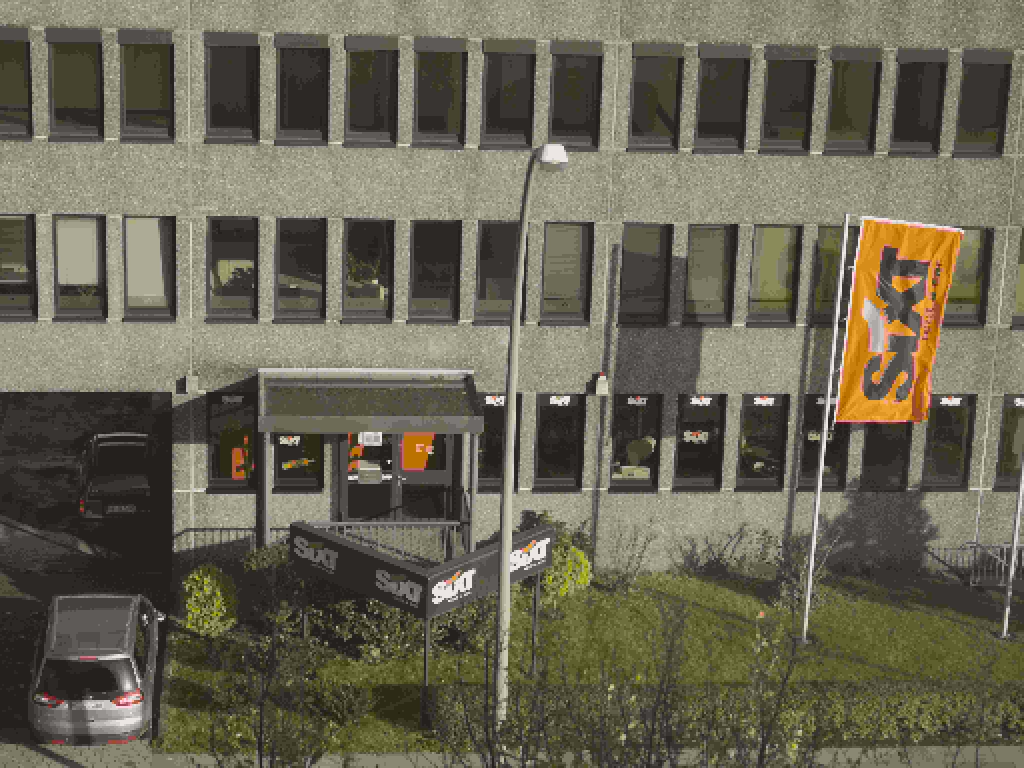
\includegraphics[scale=.23]{./res/sample_image/decompressed2.png}
				\caption*{bitrate: 0.6835, PSNR: 27.2617}
				\vspace{10pt}
				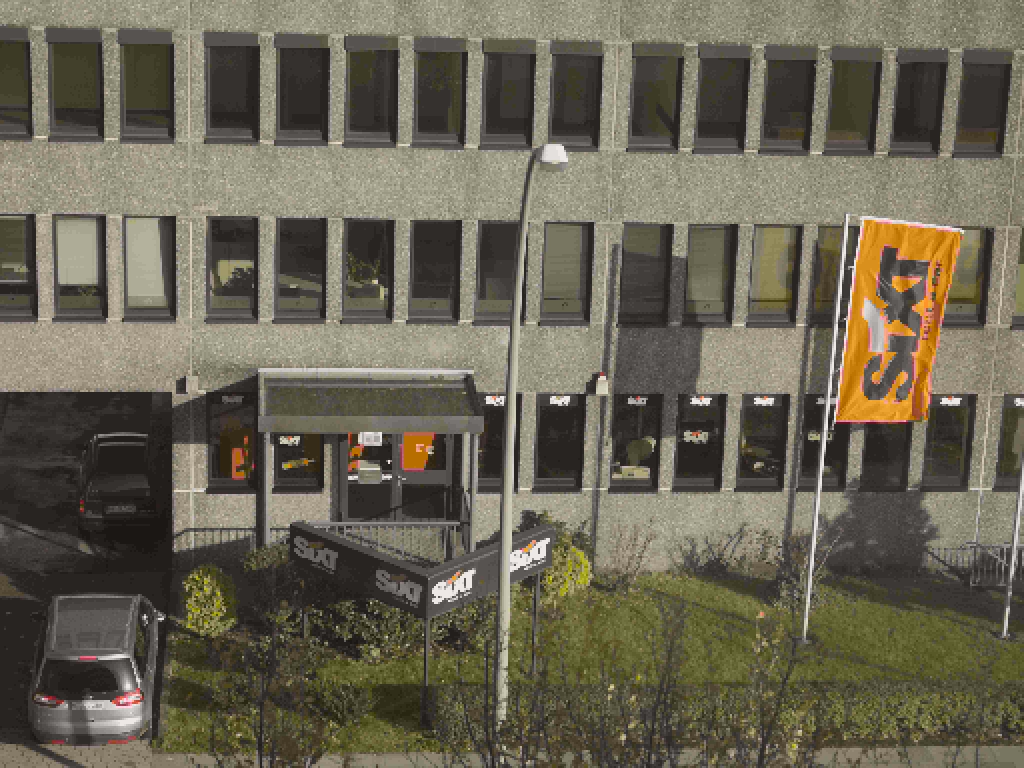
\includegraphics[scale=.23]{./res/sample_image/decompressed3.png}
				\caption*{bitrate: 0.9608, PSNR: 27.5097}
			\end{minipage}
		\end{figure}
		
	\newpage
	\item BD curve (note that the real encoded file/bitrate is always slightly smaller)
		\begin{figure}[ht]
			\hspace{-5em}
			\begin{minipage}[c]{0.6\linewidth}
				\centering
				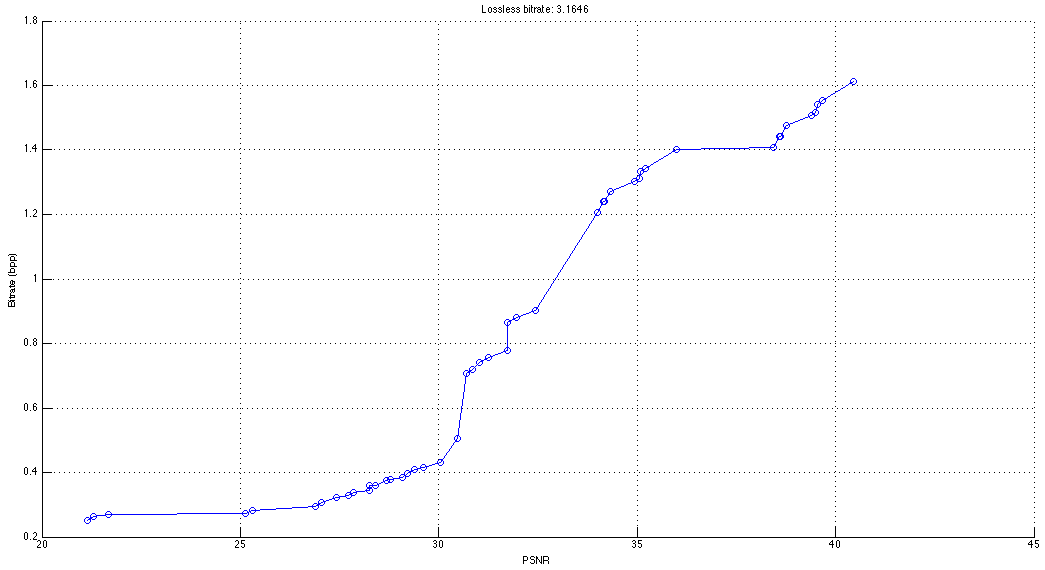
\includegraphics[scale=.28]{./res/BD_curve/BD1.png}
				\caption*{\href{https://github.com/HW-Lee/ImageCodec/blob/master/results/1_1536x1024/original.png}{Image 1 (hyperlink)}}
				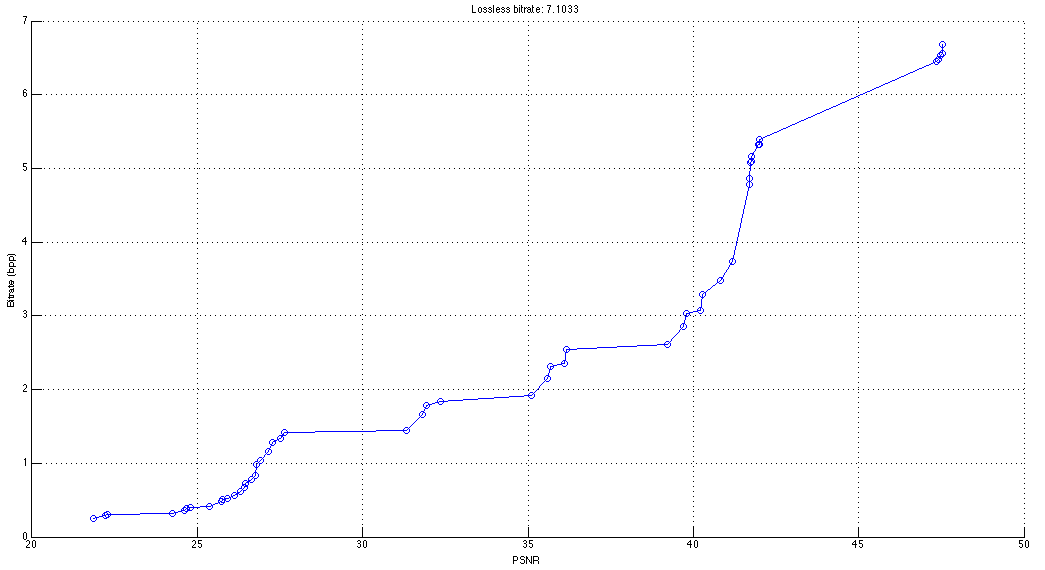
\includegraphics[scale=.28]{./res/BD_curve/BD3.png}
				\caption*{\href{https://github.com/HW-Lee/ImageCodec/blob/master/results/3_1000x728/original.png}{Image 3 (hyperlink)}}
			\end{minipage}
			\hspace{0.5em}
			\begin{minipage}[c]{0.6\linewidth}
				\centering
				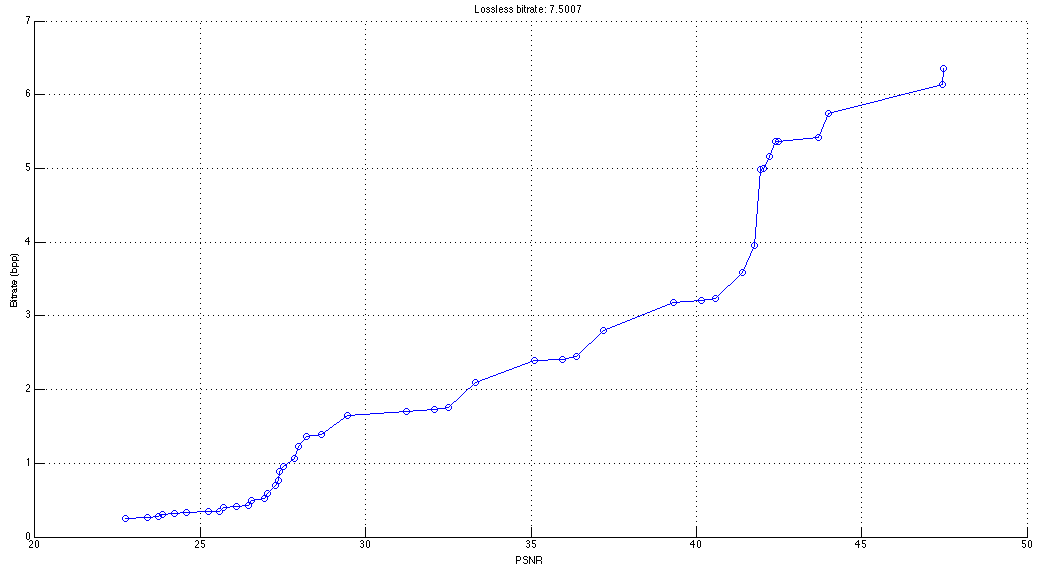
\includegraphics[scale=.28]{./res/BD_curve/BD2.png}
				\caption*{\href{https://github.com/HW-Lee/ImageCodec/blob/master/results/2_1024x768/original.png}{Image 2 (hyperlink)}}
				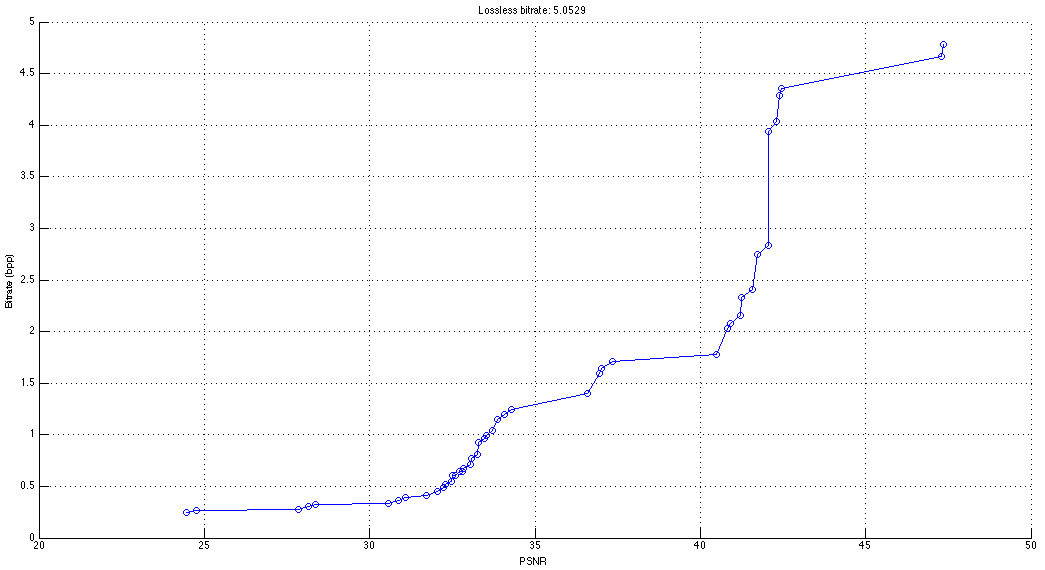
\includegraphics[scale=.28]{./res/BD_curve/BD4.png}
				\caption*{\href{https://github.com/HW-Lee/ImageCodec/blob/master/results/4_1000x1504/original.png}{Image 4 (hyperlink)}}
			\end{minipage}
		\end{figure}
		\vspace{10em}
		\begin{figure}[ht]
			\vspace{-11em}
			\centering
			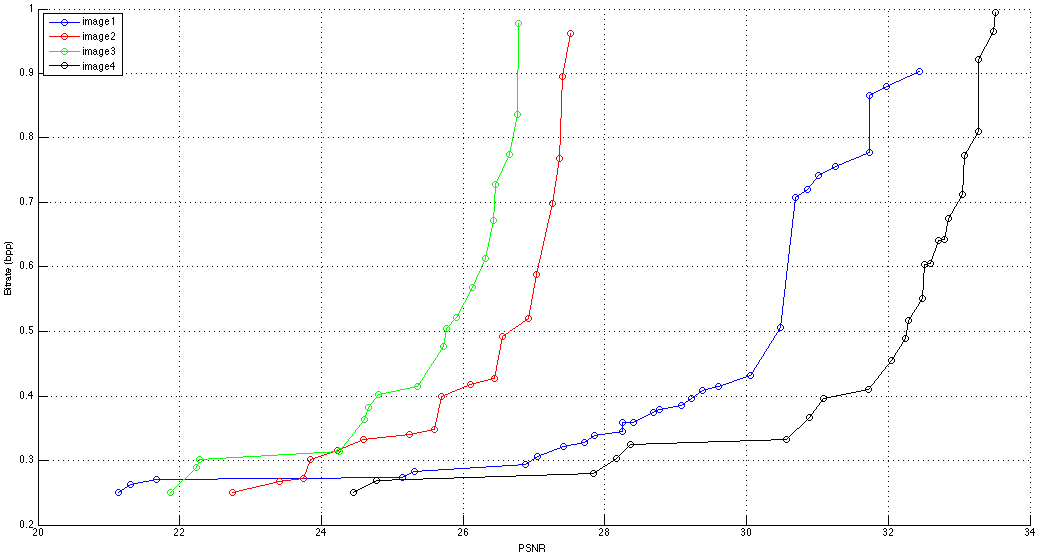
\includegraphics[scale=.5]{./res/BD_curve/BD_overall.png}
			\caption{All images where bpp is ranged from 0 to 1}
			\vspace*{-5em}
		\end{figure}
\end{enumerate}

\newpage
\section*{Discussion}
\vspace{-20pt}
\noindent\makebox[\linewidth]{\rule{\textwidth}{0.4pt}}

\begin{enumerate}
	\item Huffman Table v.s. Golomb-Rice Table
		\begin{flushleft}
			Huffman Table requires larger time consumption ($O(n^2)$), and it is powerful after seeing all data to be compressed. On the other hand, Golomb-Rice Table requires less ($O(n)$), and can be constructed without seeing any contents (fast, easily reusable). However, Huffman Table is able to fit any distribution (because it constructs itself after seeing data) and thus reach a better compression ratio. After all, this project is not focused on time consumption. Therefore, Huffman table is employed finally.
		\end{flushleft}
	\item Transform Coding
		\begin{flushleft}
			In practice, data after DCT has lower entropy than those after prediction, generally, but just saves about 10\% bitrate. Due to considerations of developing time and project variations, it is just implemented but not applied. In addition, prediction is an operation similar to decorrelation, so we expect the efficiency of DCT will not be significant. Finally, DCT is not used.
		\end{flushleft}
\end{enumerate}


\section*{Supplementary and Links}
\vspace{-20pt}
\noindent\makebox[\linewidth]{\rule{\textwidth}{0.4pt}}

\begin{enumerate}
	\item Quick start and APIs: \href{https://github.com/HW-Lee/ImageCodec/blob/master/README.md}{https://github.com/HW-Lee/ImageCodec/blob/master/README.md}
	\item References: \href{http://sun.aei.polsl.pl/~rstaros/papers/s2006-spe-sfalic.pdf}{http://sun.aei.polsl.pl/~rstaros/papers/s2006-spe-sfalic.pdf}
	\item Presentation slides:
\end{enumerate}

\end{CJK}
\end{document}